\section{Proposed model}
\subsection{Introduction}
Image-to-text conversion is a popular field in artificial intelligence that involves converting images into textual data. This technology has various applications, such as image indexing, content-based image retrieval, and image search engines. In this project, we propose a deep learning model for accurate image-to-text conversion. In this project, we aim to evaluate the performance of our proposed model using the BLEU score and conduct a comparative analysis with other state-of-the-art models. We also plan to explore the applications of our model in image indexing, content-based image retrieval, and image search engines. Overall, our proposed model has the potential to significantly improve the accuracy and efficiency of image-to-text conversion.

\subsection{Feasibility Study}
Image-to-Text Conversion Model in this feasibility study, we evaluate the feasibility of our proposed deep learning model for accurate image-to-text conversion.
\subsubsection{Technical Feasibility:}
Our proposed model involves using a pre-trained CNN as the feature extractor and an LSTM network as the text generator. Both CNN and LSTM networks have been extensively studied and proven effective in various deep learning tasks. The integration of these two components in our model is technically feasible and has been demonstrated in other state-of-the-art models.
\subsubsection{Economic Feasibility:}
The cost of implementing our proposed model depends on the availability of resources and the amount of data required. However, with the availability of publicly available datasets and cloud-based computing resources, the cost of implementing our proposed model is reasonable.

\subsubsection{Resource Feasibility:}


Deep learning models require significant computing resources, such as high-performance GPUs, to train and optimize the model. However, with the availability of cloud-based computing resources, such as Google Colab and Amazon Web Services, it is feasible to access the required computing resources at a reasonable cost.


\subsection{Requirement Analysis: }
\begin{enumerate}

  \item Data Collection: First, gather a big collection of photos, item names, and audio descriptions. This collection should include a variety of visuals blind people see every day.

  \item Data Collection: First, gather a big collection of photos, item names, and audio descriptions. This collection should include a variety of visuals blind people see every day.

  \item Machine Learning Model: The ItOD-AD system uses a dataset-trained machine learning model to detect items in photos and produce audio descriptions. A CNN model trained on the dataset to detect objects in photos powers the ItOD-AD system. The model should handle noisy, low-resolution photos and be accurate and fast.
  
\item Training: After designing the machine learning model, train it on the dataset. This entails feeding the model batches of pictures and labels and modifying its parameters to reduce the error between predicted and actual labels.
\item Validation: After training, the machine learning model must be verified on a fresh dataset to guarantee it can generalize well to new pictures.
\item Integration: Lastly, the CNN model must be connected with the ItOD-AD audio description component. The CNN model generates natural language descriptions of items in photos and delivers them to the user in a timely and accessible way.


Analyzing the requirements for your AI project of converting images to text.
Input images: The first requirement is the input images. Your model should be able to take in various types of images such as scanned documents, photos, and screenshots.
Text Extraction: The main functionality of the model is to extract text from the input image. It should be able to recognize different font styles, sizes, and colors.
Accuracy: The accuracy of the model is critical. It should be able to extract text accurately, even from low-quality images. The model should also be able to handle different languages and character sets.
Speed: The model should be able to process images quickly, especially if it needs to handle large amounts of data.
Data Storage: The model should be able to store the extracted text data efficiently for further processing or analysis.
User Interface: Your model should have a user interface that makes it easy for users to upload and process images.
Accessibility: The model should be accessible to users of all levels, including those with limited technical skills.
Security: Your model should be secure, and data privacy should be a top priority. It should be able to handle sensitive data such as bank statements, medical reports, and legal documents.
Scalability: The model should be able to handle a growing number of users and an increasing amount of data.
Cost: The cost of implementing and maintaining the model should be considered. After analyzing the requirements, you can start to develop the proposed model for image to text conversion.

\subsection{System Design:}
\begin{figure}[htbp]
\centerline{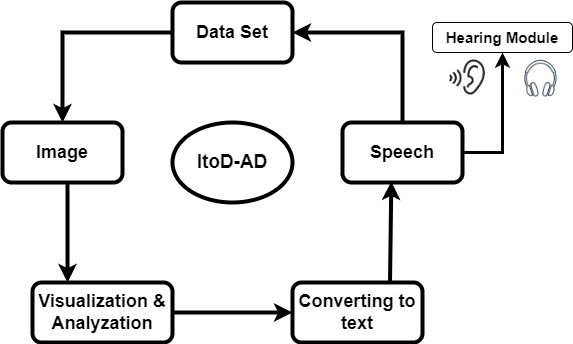
\includegraphics[width=0.5\textwidth,height=0.3\textwidth]{pic 1.jpg}}
\caption{Data flow diagram of the syetem.}
\label{fig}
\end{figure}
The machine learning-powered solution, ItOD-AD, has the ability to recognize objects in an image and produce a comprehensive audio description of the surrounding scene. By employing advanced deep learning techniques, the proposed solution can accurately identify the objects by visualization \& analyzation and generate an audio description accordingly. The implementation of ItOD-AD has the potential to greatly enhance the self-sufficiency and self-reliance of visually impaired people by providing them with real-time access to visual information.


\subsection{Implementation:}

The proposed model for image to text conversion involves several implementation steps. The first step is data collection, where a large dataset of images containing text is collected to train and test the model. The second step is model training, where a deep learning framework such as TensorFlow or PyTorch is used to train the model. The third step is model evaluation, where the performance of the model is evaluated using a test dataset. Once the model is trained and evaluated, it is deployed to a cloud platform where it can be accessed by users through a user interface. Security measures such as data encryption and access control are implemented to protect user data. The model's performance is monitored to scale up the resources as needed to handle a growing number of users and data. Finally, cost optimization measures are implemented to reduce the cost of running the model by using cost-effective resources and monitoring usage patterns. Overall, the implementation of the proposed model involves a series of steps to ensure accuracy, speed, security, and scalability, while keeping the cost low.  

\subsection{Conclusion:}
The proposed image-to-text system using deep learning techniques provides an effective solution for automatically generating text descriptions of images. The system has the potential to be applied to a variety of applications, such as image search, image retrieval, and image captioning. Further research could explore ways to improve the performance of the system and extend its capabilities to other domains.

